\chapter{\geant Simulations}
\label{chap:G4Simulation}

In High Energy Physics as well as in other reasearch areas, simulations are a tool that has become indispensable. They are used to provide model predictions, a guideline for an analysis as well as for optimising cost and performance of detector designs. In this thesis, the simulations will be used as a guideline for the selection of specific events of the recorded data. An understanding of their functionning is useful and will be described in this chapter.

\section{Simulation of particle showers}

The \geant framework \cite{Agostinelli2003} is a common toolkit in particle physics to simulate particle interactions with matter for a wide range of energies. Within this thesis, the simulations of CALICE calorimeter prototypes and the ILD detector concept are used in conjunction with the \mokka \cite{Freitas2003} and \ddhep \cite{Frank2014} framework. These frameworks provide a variety of tools for the implementation of detector geometries. \geant offers various tools and models to simulate physics processes in particle showers.

\subsection{Electromagnetic shower models}

Electromagnetic showers are generally well understood. This is mainly due to the fact that only electrons, positrons and photons are involved and their interaction with matter is simple as described in section \ref{}. All EM interactions are simulated with a standard EM package in \geant \cite{Ivanchenko2010}. This packages has been extensively compared to many observables measured in calorimeters to a level of $\leq$ 1\% \cite{Apostolakis2015}.

Recently additions have been made to the \geant EM physics list by improving the description of ionisation processes in the active medium. Then the EM list is used with a suffix \_{}EMY. This is needed in order to correctly simulate thin active layers where the detection method is very sensitive to the primary ionisation, like in gas detectors such as RPCs. The use of the \_{}EMY suffix in the EM physics list is greatly improving the agreement between data and simulation in the RPC based CALICE calorimeter prototypes, the SDHCAL and DHCAL \cite{Neubueser2016}. Many other suffix options are available depending on the type of physics, detector and precision needed for EM processes.

\subsection{Hadronic shower models}

Hadronic showers are more complex in many ways than EM showers mainly due to the compositeness of the projectile as well as the target nucleus. High energy interactions between these lead to a very large phase space in the final state. The interaction is governed by the strong force and generally cannot be solved analytically. Instead models are used using approximations and parametrisations mainly derived by theory and matched to data. Significant work has been made in the last few years in improving the modelisation and accuracy of such models. The CALICE Collaboration has been of a great help in contributing to these improvements \cite{Adloff2013, Bilki2015}.

The scale of the interaction in hadronic showers is generally given by the variable $\lambda_{B} = \frac{h}{p}$ called the De Broglie wavelength. This simple variable become shorter as the particle energy increases thus smaller structures inside a nucleus become more relevant for the description of the interaction. \geant provides several cascade models that are valid over various energy ranges. These models are described in the following.

\subsubsection{Intra-Nuclear Cascade Models}

For particle energies above a few hundred MeV and below a few GeV, the quark substructure of the nucleus is irrelevant. In this case, the interaction can be described by cascade models (see figure \ref{fig:cascademodel}). Several models are available in \geant and will be described in the following.\\

\begin{figure}[htbp!]
  \centering
  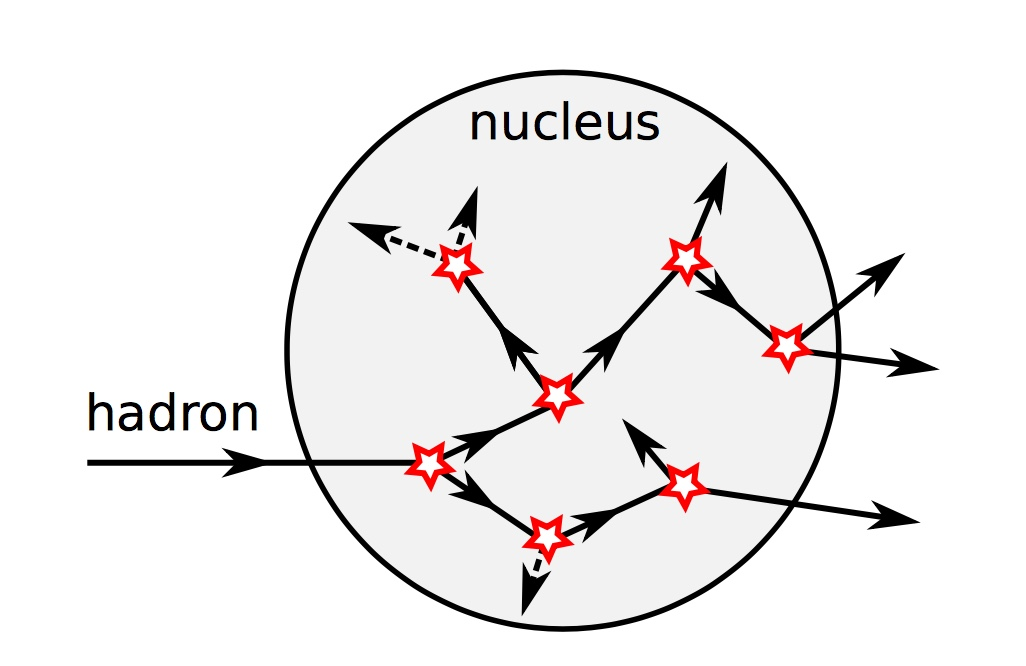
\includegraphics[width=0.5\linewidth]{chap4/fig/CascadeModel.jpeg}
  \caption{Schematic of the cascade model. The incoming projectile and all secondaries inside the nucleus are tracked and their interaction is calculated until they are under a certain threshold or leave the nucleus. Taken from \cite{Feege2011}.} \label{fig:cascademodel}
\end{figure}

\textbf{Bertini Cascade}\\

The Bertini cascade model \cite{Heikkinen2003} consists of the modelisation of a nucleus by three concentric spherical shells of approximative constant nucleon density. The nucleons are treated as a degenerated Fermi gas in each shell and all energy levels are filled up to the Fermi energy ($E_F$). Following the Pauli exclusion principle that products can't be in an occupied state (lowest level filled by the Fermi gas), only secondary nucleons of energy $E > E_F$ can be produced. During the intra-nuclear cascade (INC), the momentum, the type of interaction and the four momentum of the interaction for each nucleon is calculated until the energy of the tracked nucleon is below 2 MeV. The INC gives rise to exited states of the nucleon thus a pre-equlibrium evaporation, as emission of protons and neutrons, is computed. Then a de-excitation model is performed including Fermi break-up of highly excited light nucleus (A < 12), explosion model, fission model and evaporation model until the excitation energy is below 0.1 MeV.\\

\textbf{Binary Cascade}\\

The Binary cascade \cite{Folger2004} is another approach to model the interaction between a projectile and a target nucleus. The model describes the nucleons with defined position and momentum following the nucleon mass, density distribution and Pauli's exclusion principle. The momentum is chosen randomly between zero and the Fermi momentum ($p_{F}^{max}(r)$) such as the total momentum of the nucleus is zero (at rest). The model is then treated by steps of excitations and decay into secondary particles emerging from the interaction until the average energy of all participants in the nucleus is below a given threshold (70 MeV). The remaining nucleus is further treated by pre-equlibrium and de-excitation models in \geant. The validity range of this model extends from around 100 MeV up to 10 GeV.

\subsubsection{String-Parton Cascade Models}

\begin{figure}[htbp!]
  \centering
  \begin{subfigure}[t]{0.49\textwidth}
    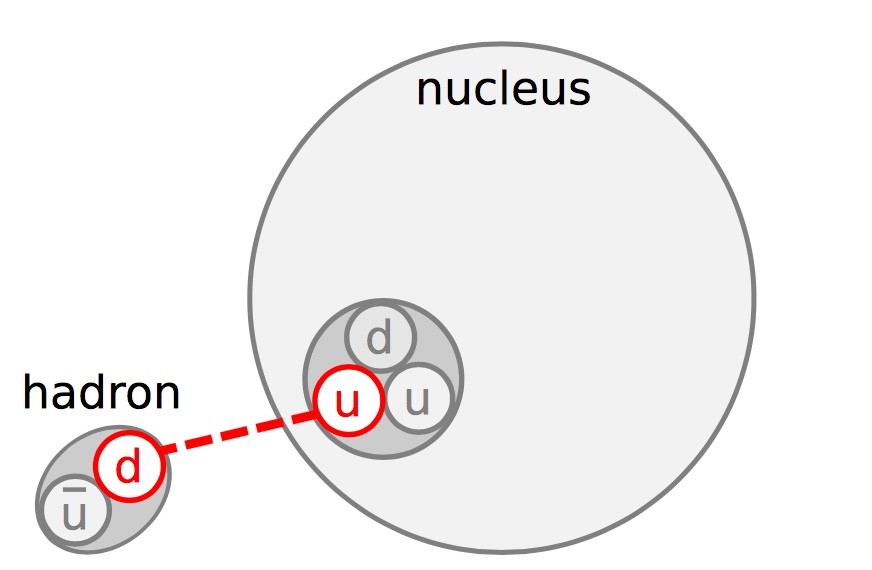
\includegraphics[width=1.\linewidth]{chap4/fig/QGS_nucleus.jpeg}
    \caption{} \label{fig:QGS_nucleus}
  \end{subfigure}
  \hfill
  \begin{subfigure}[t]{0.49\textwidth}
    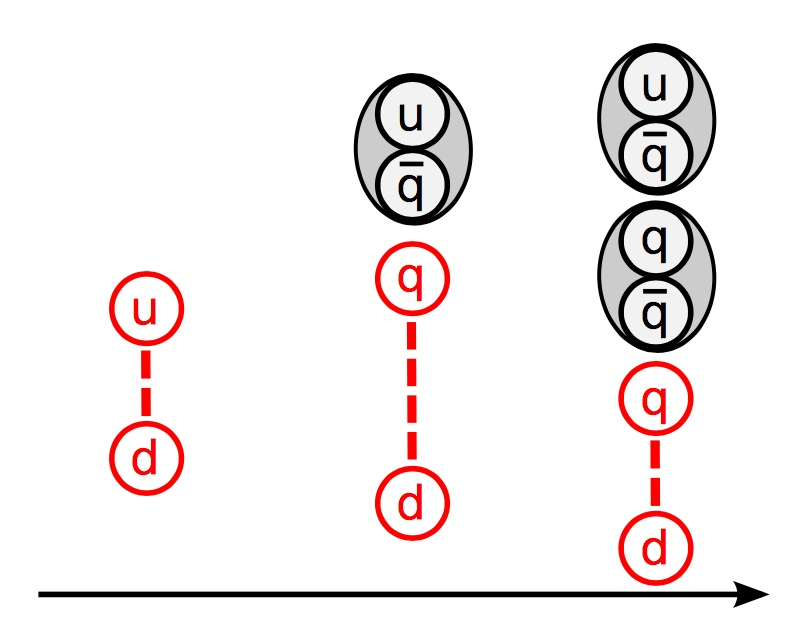
\includegraphics[width=1.\linewidth]{chap4/fig/QGS_stringfrag.jpeg}
    \caption{} \label{fig:QGS_string}
  \end{subfigure}
  \caption{\subref{fig:QGS_nucleus}) The sketch shows the formation of a string between the projectile and one of the quarks inside the nucleus. \subref{fig:QGS_string}) Representation of the fragmentation of the strings via the generation of quark-antiquark pairs into hadrons. Taken from \cite{Feege2011}.}
\end{figure}

The string-parton models \cite{Folger2003} are used in \geant to simulate inelastic scattering of particles with a target nucleus as shown in figures \ref{fig:QGS_nucleus} and \ref{fig:QGS_string}. This is used at high energies where INC models break down and where the quark substructure of the nucleons must be taken into account. The model uses string excitation to calculate the scaterring. Currently, \geant provides two different models, the Fritiof model (FTF) and the quark gluon string model (QGS). The latter will be described in the following.

The initial state consists of building the nucleus of individual protons and neutrons. The interaction between the primary particle and the nucleus gives place to one or more excited strings and a excited state nucleus. A string has two endpoints, such that the quark content is defined and caries energy and momentum. The fragmentation of the strings is handled by a longitudinal string fragmentation model and the interaction of secondaries is carried out by cascade models as described in the former paragraph. The de-excitation is then simulated by fragmentation, pre-compound and nuclear de-excitation models natively provided by \geant. The QGS model uses longitudinal strings to represent the momentum transfer and tranverse strings for color exchange via Pomerons. In contrary, the FTF model uses an interaction probabilty calculated based on impact parameter, center of mass energy, diffractive and elastic cross-sections to form a string.

\subsection{\geant Physics Lists}

\geant provides several physics lists for simulation that combine different hadron physics models. In this thesis, the physics lists QGSP\_BERT and QBBC are used. The validity range of the physics lists is shown in figure \ref{fig:physics_list}. The former is used in combination with the High-Precision neutron tracking (HP) package. The HP option delivers an increased accuracy in the treatment of neutron interactions below 20 MeV. The QBBC physics list possesses a comparable tracking for neutrons with less precision.
In addition, the QGSP\_BERT physics list uses a parametrised LEP model (based on expirimental data) to fill the gap between the transition of cascade models and string-parton models.

\begin{figure}[htbp!]
  \centering
  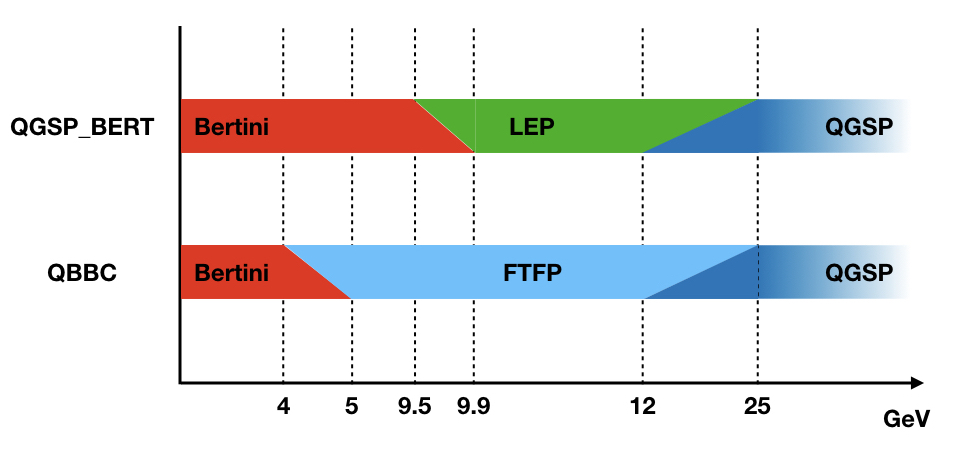
\includegraphics[width=1\linewidth]{chap4/fig/PhysicsLists.jpeg}
  \caption{Schematic of the physics list used in \geant v10.1 for this thesis. The validity range extends over 30 GeV.} \label{fig:physics_list}
\end{figure}

\section{AHCAL Detector Geometry implementation and Digitisation}

\subsection{Geometry implementation}

The simulation of the testbeam prototype is based on the \mokka framework v08-05-01 and the new \ddhep framework v00-16, which both provide a full \geant v10.1 based simulation of the detector with detailed geometry and material descriptions. A right handed coordinate system is used such that the Z-axis points in the beam direction and that the Y-axis is directed upwards. No beamline instrumentation is simulated except scintillator triggers in front of and behind the detector. An additional layer of 5.6 mm of lead (corresponds to 1 $X_0$) is added in front of the calorimeter in order to account for missing upstream material. This analysis uses the sub-detector \mokka models \textit{TBecal4d} for the ScECAL (Scintillator strips with EBUs) and \textit{TBhcal4d} for the AHCAL. The distance between the sub-detectors is set to 0 mm. A picture of the model in DD4hep is shown in figure \ref{fig:GeomModel}. A check was performed with \mokka and \ddhep models with muons and electrons to ensure that the material description in both models are better than 20\% (see section \ref{appendix:SimulationVal}).\\

The beam gun is placed 1 m in front of the calorimeter face for the simulations in this analysis. It is configured to generate single beam particles with a 2\% momentum spread (according to the beamline) and the beam profile for electrons and pions is extracted from data and applied to simulation. For muon runs, a flat beam covering the full AHCAL is simulated as this is not expected to have an influence on the MIP and time response of the detector. All electron simulations are simulated with \geant 10.1 using the QGSP\_BERT\_HP physics list.\\

Pion showers are simulated using QGSP\_BERT, QGSP\_BERT\_HP and QBBC physics lists. The package \textit{high precision} (\_HP) is used in order to understand the differences induced in timing with a precise treatment of the neutrons. In this analysis, 1000000 simulated 150 GeV $\mu^-$, 20000 from 15 to 40 GeV $e^-$, 200000 10 and 50 GeV $e^-$ and 500000 from 10 to 90 GeV $\pi^-$ single particle events are generated.

\begin{figure}[htbp!]
  \centering
  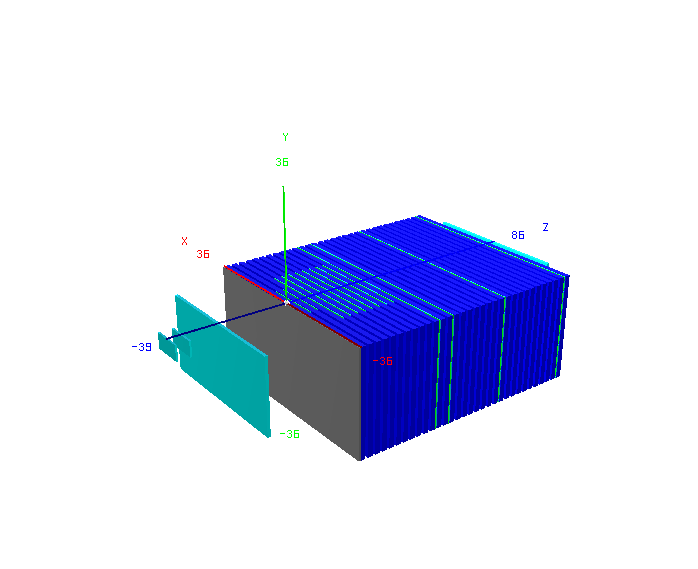
\includegraphics[width=0.7\linewidth]{chap4/fig/DD4hep_AHCALModel.png}
  \caption{DD4hep geometry model of the 2015 testbeam prototype.} \label{fig:GeomModel}
\end{figure}

\subsection{Digitisation}

The digitisation of simulated hits is very similar to the one used in the ScECAL and AHCAL physics prototypes \cite{2011_JINST_6_P04003}. First, the energy deposited in a cell is converted in MIP. The conversion unit named \textit{GeVtoMIP} is extracted from simulation by projecting 8 GeV muons onto a detector tile and fitting the resulting spectrum with a landau function. Motivated by physics, as explained in section \ref{}, idealy for a thin active material, the energy deposited follow a Landau distribution. The MPV of this dribtribution is used as the \textit{GeVtoMIP} factor. For this setup, a value of 470 keV is used for the AHCAL and 309 keV for the ScECAL.\\

Using, if available, individual calibration factors obtained from data to extract the light yield which is needed to model the statistical fluctuations of photons hitting a SiPM \cite{Hartbrich:2016bbz}. Saturation effects are also included using the number of pixels available on each SiPM type. Most of the tiles used are wrapped with a reflective foil such that crosstalk effects between channels can be neglected. For layers with no wrapping a default value of 15\% cross-talk is applied. Additionally, noise needs to be taken into account for the engineering AHCAL prototype. It is to point out that noise is much lower than in the physics prototype but it is important to be taken into account for this thesis as timing is very sensitive to low statistics late tails. Noise is added using muon runs by removing found tracks and keeping remaining hits. This is described in appendix \ref{appendix:noise}.\\

The timing is modelled in the same way as in the SPIROC, the energy from sub-hits in a cell is integrated over a sliding time window of 15 ns, if the energy sum passes the threshold the time of the simulated sub-hit passing the threshold is registered as the time of the hit. In order to simulate detector resolution effects, the time of a hit is smeared with a double gaussian function with slightly different means and sigmas convoluted with a gaussian of fixed mean and variable sigma. More details are explained in appendix \ref{appendix:ped_shift}.\\

After digitisation, simulated hits have the same format as raw data hits and are then reconstructed using the same software chain as is used for data. To suppress noise, only hits above 0.5 MIP are considered in this analysis in both simulation and data.
